\documentclass[12pt]{article}
\usepackage{caption}
\usepackage{float}
\usepackage{graphicx}
\usepackage{fancyhdr}
\pagestyle{fancy}
\pagenumbering{Roman}
\renewcommand{\headrulewidth}{1pt}
\renewcommand{\footrulewidth}{1pt}
\setlength{\headheight}{25pt}
\rhead{\textbf{Lightning Coalition Robotics}}
\cfoot{}
\rfoot{\thepage}
\begin{document}

% Add date (e.g. September 14, 2018) and then your name/all authors.
January 5, 2019 - Nathaniel Smith

\section{Our Plan:} % Pretty self explanatory... In this section explain the team's plan.
\begin{itemize}
% After \item, add what you want for the bullet point. (\item adds a new bullet point when you run out.)
	\item design t-shirts
\item create biographies
\item program autonomous
\item program tele-op for remote controller
\item make mineral holding device
\item work on the collection mechanism
\item work on the Stronk Boi
\end{itemize}

% Now add a paragraph explaining your plan. You should reference the bullet points above.
We will design the t-shirts in preparation for the competition. We plan for our members to create biographies of themselves so that we can give them to the judges. We plan to work on programming the autonomous code for the first part of the contest. We also plan to work on programming the tele-op code for the remote controller that we will use in the second part of the contest. We also plan to work on the mineral holding device that we will use to store up to two minerals in the contest. We also plan to work on the collection mechanism because it will be useful to pick up minerals. We will also work on constructing the Stronk Boi because we will use it to raise and lower the robot from the lander during the contest.

\section{What We Got Done:} % Just like the above, explain what the team got done during practice.
\begin{itemize}
% After \item, add what you want for the bullet point. (\item adds a new bullet point when you run out.)
	\item worked on scouting spreadsheet
\item we mounted the spool for the Stronk Boi and strung it up
\item we worked on designing the t-shirts
\item we have been trying to fix certain problems in the code
\item started the outreach
\item worked on building the mineral holding device
\item we modified the Stronk Boi to fix problems
\end{itemize}

% Now add a paragraph explaining what you got done and the reasons behind it. You should reference the bullet points above.
Today we worked on the scouting spreadsheet because one of our members focused on it. We were also to string up the Stonk Boi and mount the spool for it so we can test the robot when it comes time. We encountered some difficulties with the Stronk Boi attaching to the lander hook, so we modified the Stronk Boi to fix it. Also, we worked on designing t-shirts and narrowed down our options so we can be prepared for the competition. Our coding was mysteriously malfunctioning, even though everything looked ok. We began working on outreach so that we can get more points during the competition. We worked on the mineral holding device so we can test it when the robot is ready.

\section{What We Didn't Get Done:} % Explain what the team didn't get done during practice.
\begin{itemize}
% After \item, add what you want for the bullet point. (\item adds a new bullet point when you run out.)
	\item we weren’t able to finish the collection mechanism
\item we weren’t able to fix the code entirely
\end{itemize}

% Now add a paragraph explaining what you didn't get done and the reasons behind it. You should reference the bullet points above.
We weren’t able to finish the collection mechanism because the robot needed to be worked on in many different ways, and they all couldn’t be done at the same time. We weren’t able to finish the fixing the code because it is very confusing and we need more time to fix it.

\section{Next Practice:}
\begin{itemize}
% After \item, add what you want for the bullet point. (\item adds a new bullet point when you run out.)
	\item we plan to restring the Stronk Boi
\item fine tune autonomous to sense the orientation images in the arena and move better
\item fix code
\item work on mineral holding device
\end{itemize}

% Now add a paragraph explaining what the plan for next practice should be. You should reference the bullet points above.
The next practice is Sunday, January 6th, 2019
We plan to restring the Stronk Boi because the fishing line that we strung it with broke. We will use paracord because it is better than fishing line since it can handle more tension. We plan to fine tune the autonomous to sense the orientation images in the arena and move better so the robot can perform more efficiently. We would also like to finish fixing the code so the robot will work properly. Finishing the mineral holding device is ideal because it is useful to the robot.

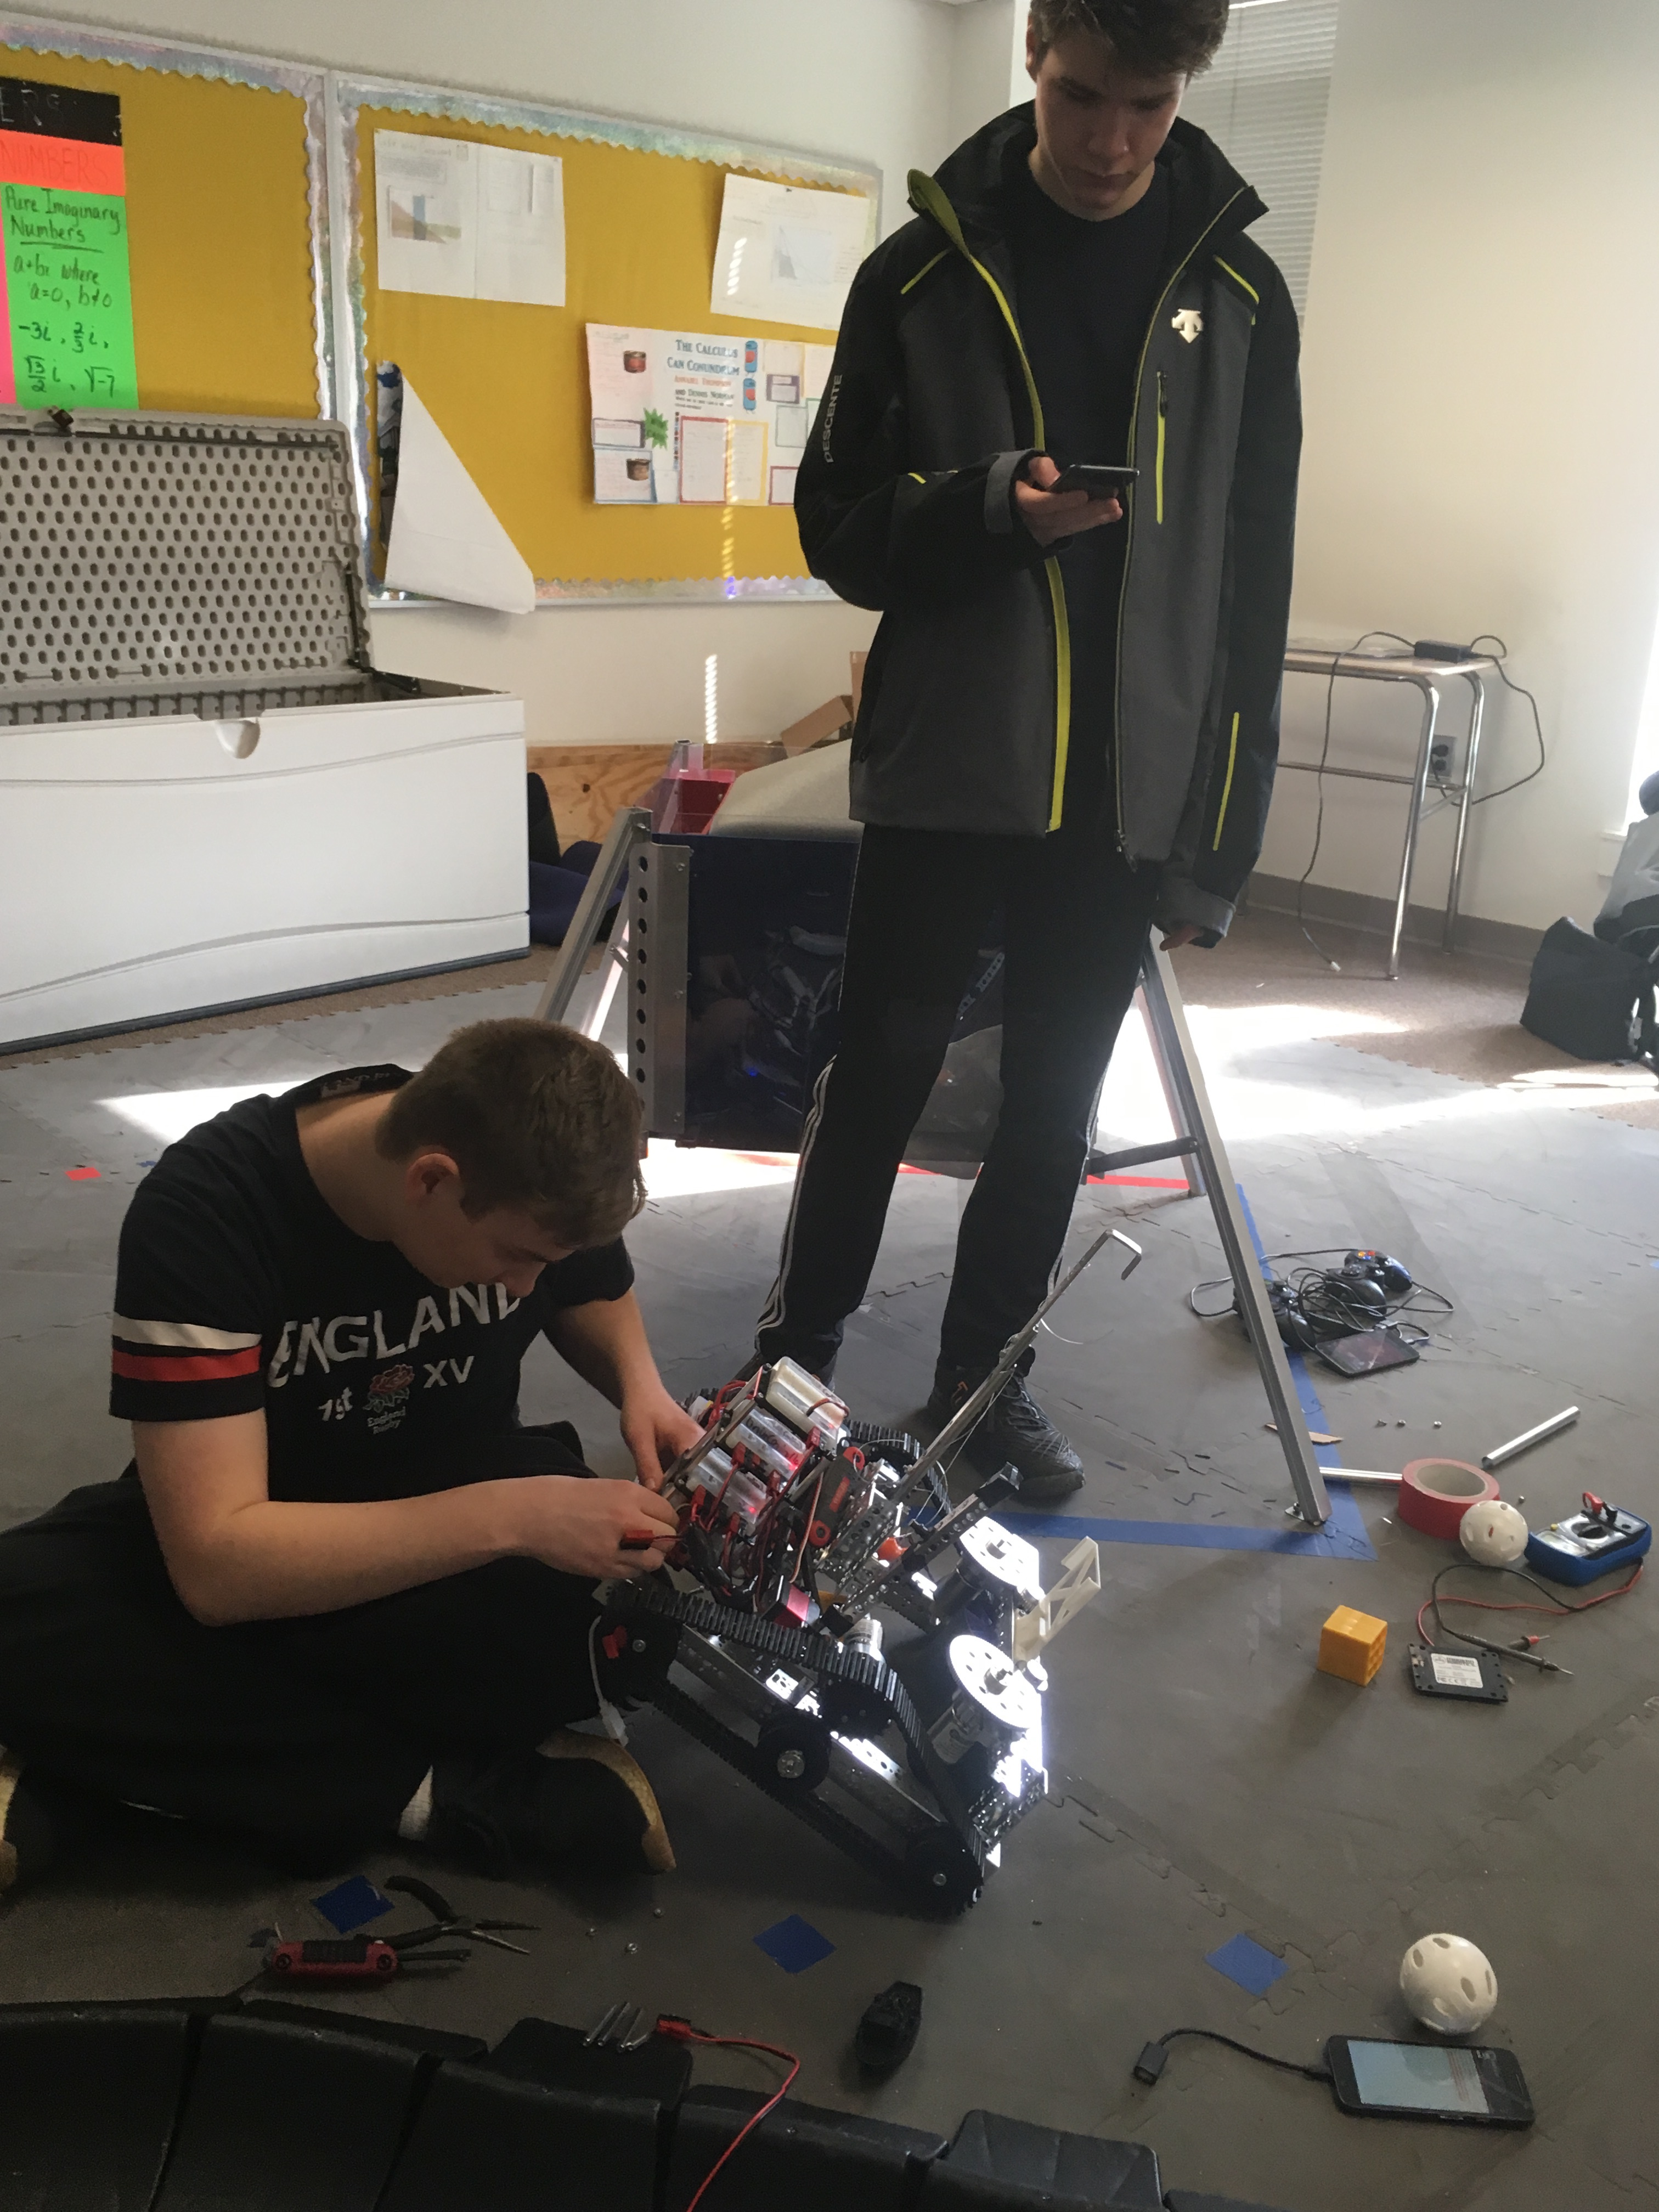
\includegraphics[width=75mm,scale=0.5]{jan5/IMG_3672}
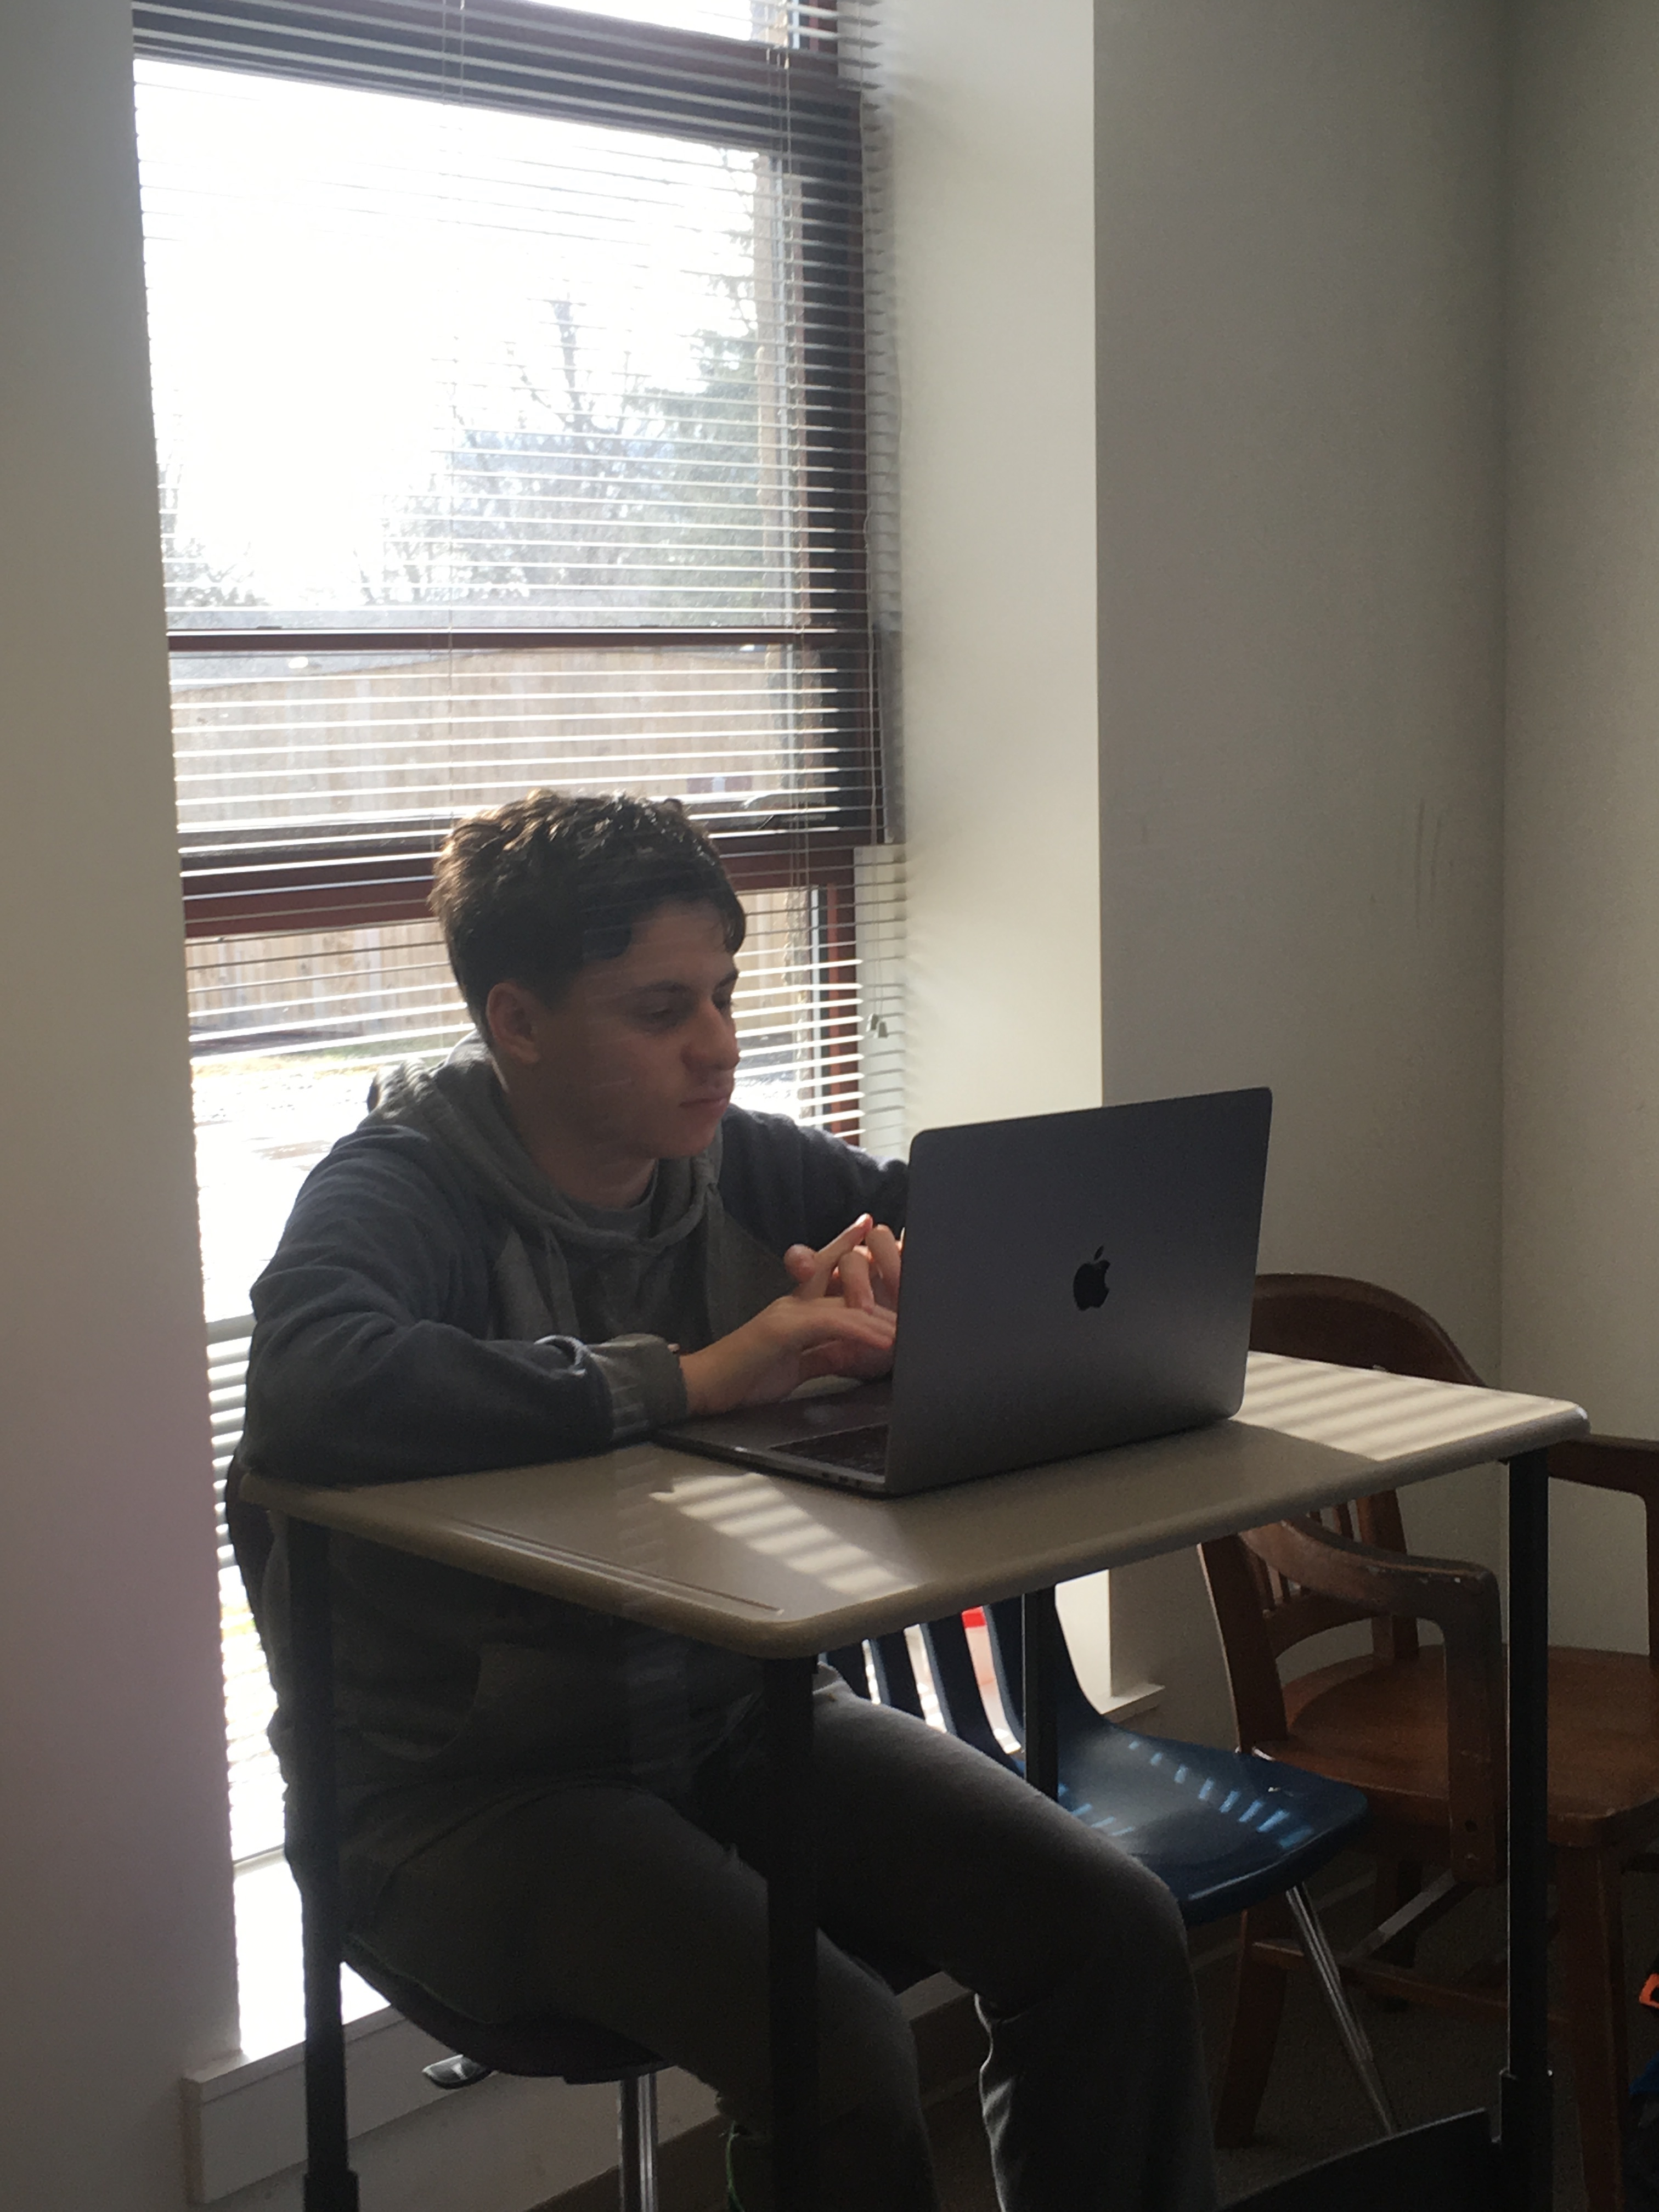
\includegraphics[width=75mm,scale=0.5]{jan5/IMG_3666}

\end{document}
